In this section we consider the case studies used to demonstrate the use of Dippy. The case studies are:
\begin{enumerate}
\item the bin packing problem;
\item the coke supply chain problem (a capacitated facility location problem within a transshipment problem);
\item the travelling salesperson problem;
\item the cutting stock problem;
\item the wedding planner problem (a set partitioning problem)
\end{enumerate}

We will define the case studies in PuLP and demonstrate their solution in \ac{DIP} without any customisation. We used \ac{DIP} version 0.9.9 and Dippy version 1.9.9.

\subsection{The Bin Packing Problem (bin\_pack\_func.py and bin\_pack\_instance.py)} \label{sbs:binpack}

The solution of the bin packing problem determines where, amongst $m$ ``bins'', to place $n$ ``items'' of various ``volumes'' in a way that (in this case study) minimises the wasted ``capacity'' of the bins. Each product $j=1, \ldots, n$ has a volume $v_j$ and each bin has capacity $C$. Extensions of this problem arise often in \ac{MILP} in problems including network design and rostering.

The \ac{MILP} formulation of the bin packing problem is straightforward. The decision variables are
\begin{align*}
x_{ij} &= \begin{cases} 1 & \text{if item $j$ is placed in bin $i$} \\
0 & \text{otherwise} \end{cases} \\
y_i &= \begin{cases} 1 & \text{if a facility is located at location $i$} \\
0 & \text{otherwise} \end{cases} \\
w_i &= \text{ ``wasted'' capacity at location $i$}
\end{align*}
and the formulation is
\[
\begin{array}{rr@{\ }ll}
       \min & \displaystyle \sum_{i=1}^m w_i \\
\text{s.t.} & \displaystyle \sum_{i=1}^m x_{ij}           & = 1, j = 1, \ldots, n      & \text{ (each product produced)} \\
            & \displaystyle \sum_{j=1}^n v_j x_{ij} + w_i & = C y_i, i = 1, \ldots, m  & \text{ (aggregate capacity at location $i$)} \\
            & \multicolumn{2}{l}{x_{ij} \leq y_i, i = 1, \ldots, m, j = 1, \ldots, n}  & \text{ (disaggregate capacity at location $i$)} \\[6pt]
            & \multicolumn{3}{l}{x_{ij} \in \{ 0, 1\}, w_i \geq 0, y_i \in \{0, 1\}, i = 1, \ldots, m, j = 1, \ldots, n}
\end{array}
\]

Note that the disaggregate capacity constraints are not necessary for defining the solution, but tighten the \ac{MILP} formulation (i.e., remove factional solutions from the solution space). Using PuLP we can easily define and solve this \ac{MILP} problem in Dippy. The formulation and solution functions from bin\_pack\_func.py are given below with a summary for each fragment.

\begin{enumerate}[leftmargin=0cm,itemindent=0.75cm,labelwidth=.5cm,labelsep=.25cm,labelindent=0cm,align=left]
\item Load PuLP and Dippy;
\lstinputlisting[firstnumber=12,linerange=12-30]{../../examples/Dippy/bpp/bin_pack_func.py}

\item Define \lstinline{BinPackProb}, a class that describes a bin packing problem;
\lstinputlisting[firstnumber=34,linerange=34-40]{../../examples/Dippy/bpp/bin_pack_func.py}

\item Define the \lstinline{formulate} function, with a bin packing problem object as input;
\begin{enumerate}[leftmargin=0cm,itemindent=0.75cm,labelwidth=.5cm,labelsep=.25cm,labelindent=0cm,align=left]
\item Create a \lstinline{DipProblem} (with some display options defined);
\lstinputlisting[firstnumber=42,linerange=42-47]{../../examples/Dippy/bpp/bin_pack_func.py}

\item Using the bin packing problem object's data (i.e., the data defined within \lstinline{bpp}), create the decision variables;
\lstinputlisting[firstnumber=49,linerange=49-54]{../../examples/Dippy/bpp/bin_pack_func.py}
\item and the objective function;
\lstinputlisting[firstnumber=56,linerange=56-56]{../../examples/Dippy/bpp/bin_pack_func.py}
\item and constraints;
\lstinputlisting[firstnumber=58,linerange=58-68]{../../examples/Dippy/bpp/bin_pack_func.py}

\vspace*{1cm} % \newpage destroys list spacing so pushing item down

\item Finally, the bin packing problem object and the decision variables are all ``embedded'' within the \lstinline{DipProblem} object, \lstinline{prob}, and this object is returned (note that the objective function and constraints could also be similarly embedded).
\lstinputlisting[firstnumber=82,linerange=82-89]{../../examples/Dippy/bpp/bin_pack_func.py}
\end{enumerate}

\item Define the \lstinline{solve} function that only requires a \lstinline{DipProblem} object, \lstinline{prob}, (note that no \lstinline{dippyOpts} are specified, so the Dippy defaults are used).
\lstinputlisting[firstnumber=123,linerange={123-124,132-132,143-148}]{../../examples/Dippy/bpp/bin_pack_func.py}

\end{enumerate}

To solve an instance of the bin packing problem, the data needs to be specified and then the problem formulated and solved as demonstrated in the file bin\_pack\_instance.py.
\lstinputlisting[firstnumber=3,linerange=3-22]{../../examples/Dippy/bpp/bin_pack_instance.py}

Solving this bin packing problem instance in Dippy gives the branch-and-bound tree shown in figure \ref{fig:bpp_tree1} (note that the integer solution found -- indicated in blue \lstinline{S: 5.0} -- bounds all other nodes in the tree) with the final solution packing items 1 and 2 into bin 0 (for a waste of 1), items 3 and 5 into bin 1 (for a waste of 3) and item 4 into bin 3 (for a waste of 1).
\begin{figure}[htp]
\begin{center}
%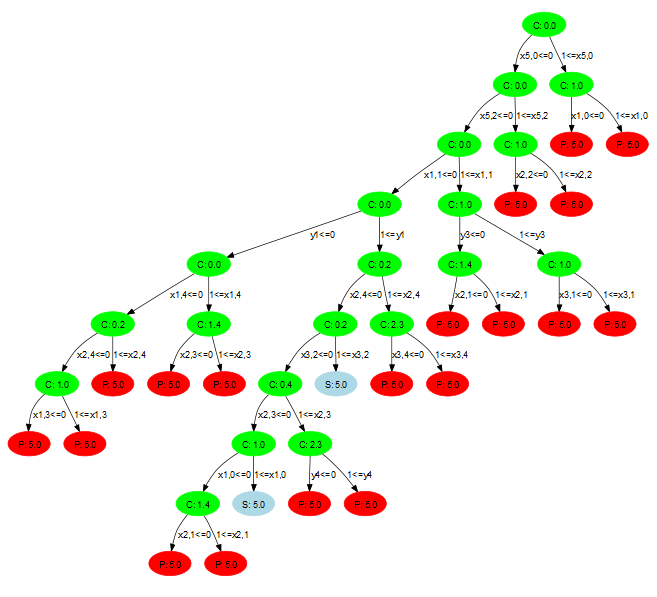
\includegraphics[bb=0 0 815 496,scale=0.50]{img/bpp_tree1.png}

\includegraphics[scale=0.16]{img/bpp_tree1.eps}
\end{center}
\caption{Branch-and-bound tree for bin packing problem instance.} \label{fig:bpp_tree1}
\end{figure}

\newpage
Note that \ac{DIP} uses cuts from the \ac{CGL} \cite{coin_or} by default. We can turn \ac{CGL} cuts off by setting the {\tt CutCGL} flag in the \lstinline{dippyOpts} to \lstinline{'0'}.
\lstinputlisting[firstnumber=134,linerange={134-135,142-143}]{../../examples/Dippy/bpp/bin_pack_func.py}
The size of the branch-and-bound tree increases significantly  as shown in \figref{fig:bpp_tree4}.
\begin{figure}[htp]
\begin{center}
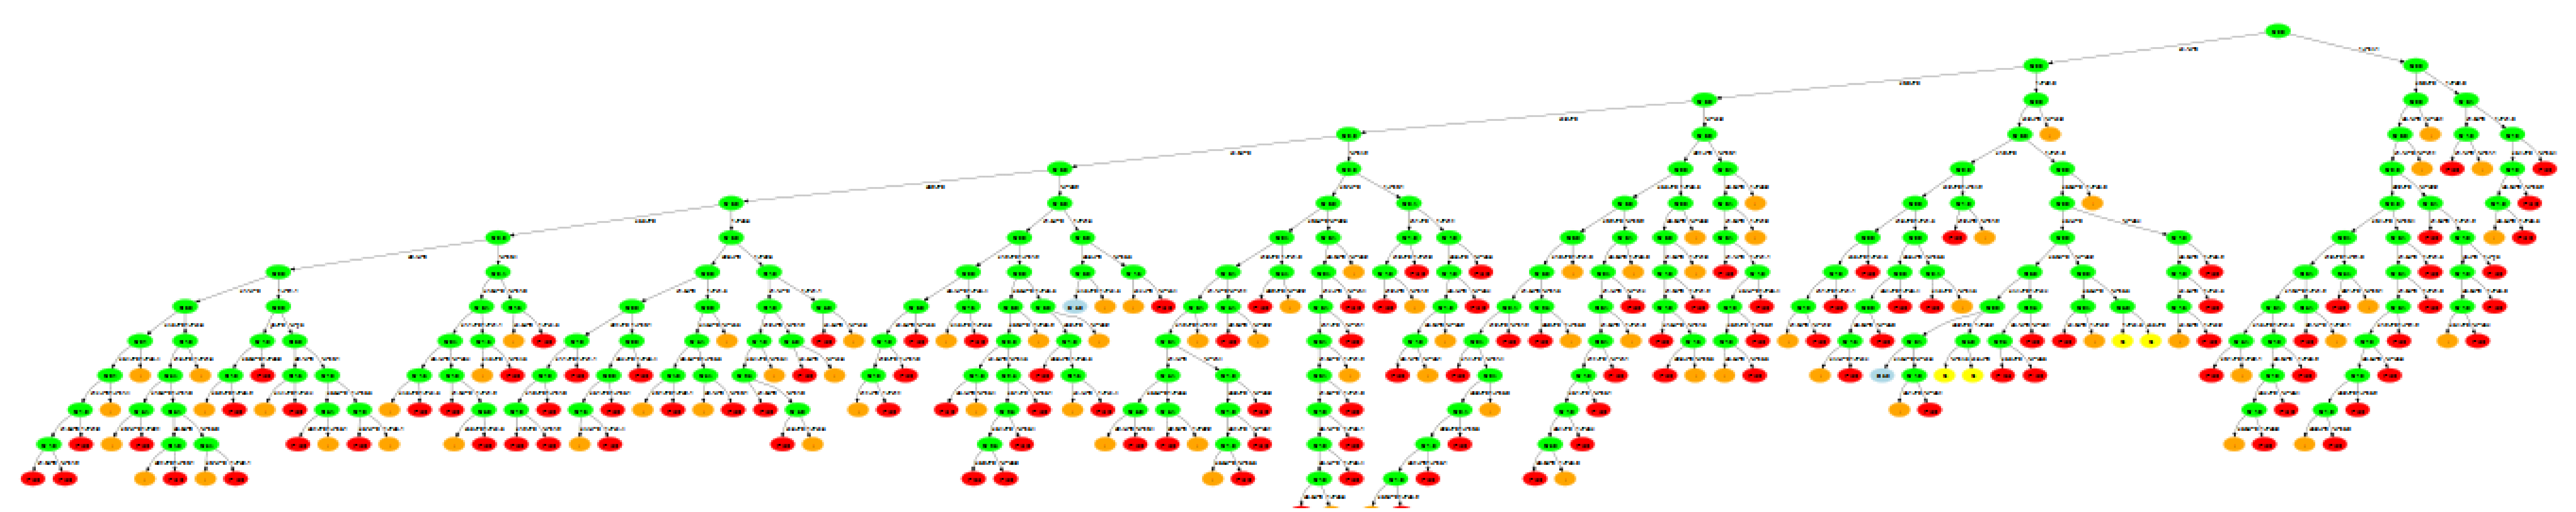
\includegraphics[scale=0.08]{img/bpp_tree4.eps}
\end{center}
\caption{Branch-and-bound tree for bin packing problem instance without \ac{CGL} cuts.} \label{fig:bpp_tree4}
\end{figure}





\subsection{The Coke Supply Chain Problem (coke\_func.py and \\ coke\_instance.py)} \label{sbs:coke}

This case study is sourced from the Operations Research Web in the Department of Engineering Science TWiki \cite{coke} (and was originally adapted from Leyland et al. \cite{geoff_coke}). There are 6 coal mines that produce coal. The coal is transported from the 6 mines to a coke-making plant where it is converted to coke using ``thermal decomposition''. Every tonne of coke produced by thermal decomposition requires 1.3 tonnes of coal. From the coke-making plants the coke is transported to one of 6 customers. There are 6 locations where coke-making plants can be constructed. There are 6 different size plants that can be constructed at each location.

The size of a plant determines the coke processing level in kilotonnes/year the plant can produce. \Tabref{tab:plant_size} shows the different plant sizes with their corresponding processing levels and construction cost in million RMB.
\begin{table}[htp]
\begin{center}
\begin{tabular}{|c|c|c|}
\hline
\multirow{2}{*}{\bf Plant Size} & {\bf Processing Level} & {\bf Cost} \\
 & {\bf (kT/year)} & {\bf (MRMB)} \\
\hline
1 & 75 & 4.4 \\
2 & 150 & 7.4 \\
3 & 225 & 10.5 \\
4 & 300 & 13.5 \\
5 & 375 & 16.5 \\
6 & 450 & 19.6 \\
\hline
\end{tabular}
\caption{Possible plant sizes} \label{tab:plant_size}
\end{center}
\end{table}

To get this problem into Dippy we use the PuLP modelling language.  The formulation and solution functions from coke\_func.py are given below with a summary for each fragment.

\begin{enumerate}[leftmargin=0cm,itemindent=0.75cm,labelwidth=.5cm,labelsep=.25cm,labelindent=0cm,align=left]
\item PuLP and Dippy are loaded in an identical way to bin\_pack\_func.py (see \scnref{sbs:binpack});

\item Define \lstinline{CokeProb}, a class that describes a coal-to-coke conversion and transportation problem;
\lstinputlisting[firstnumber=26,linerange=26-41]{../../examples/Dippy/coke/coke_func.py}

\item Define the \lstinline{formulate} function, with a bin packing problem object as input;
\begin{enumerate}[leftmargin=0cm,itemindent=0.75cm,labelwidth=.5cm,labelsep=.25cm,labelindent=0cm,align=left]
\item Create a \lstinline{DipProblem} (with some display options defined);
\lstinputlisting[firstnumber=43,linerange=43-49]{../../examples/Dippy/coke/coke_func.py}

\item \label{itm:2d} Define a 2-dimensional set for the plant sizes at each location;
\lstinputlisting[firstnumber=88,linerange=88-89]{../../examples/Dippy/coke/coke.py}

\item Create a \texttt{DipProblem} (extended from \texttt{LpProblem} in PuLP). Add binary variables that determine the plant sizes at each location and (non-negative) integer variables that determine the flow (in coal from the mines to the plants and coke from the plants to the customers) transported through the network;
\lstinputlisting[firstnumber=91,linerange=91-99]{../../examples/Dippy/coke/coke.py}

\item Add the objective of minimising total cost = building costs (converted from MRMB to RMB) + transportation costs;
\lstinputlisting[firstnumber=101,linerange=101-106]{../../examples/Dippy/coke/coke.py}

\item Add constraints that limit the flow of coke out of a coke-making plant depending on the capacity plant constructed;
\lstinputlisting[firstnumber=108,linerange=108-113]{../../examples/Dippy/coke/coke.py}

\item Add constraints that limit the number of coke-making plants built at any single location to be one (Note. there is a size with capacity 0 if no plant will be built);
\lstinputlisting[firstnumber=115,linerange=115-118]{../../examples/Dippy/coke/coke.py}

\item Add constraints to conserve flow at the mines ($\leq$ supply), coke-making plants (flow in = coke-from-coal conversion rate $\times$ flow out) and customers ($\geq$ demand);
\lstinputlisting[firstnumber=120,linerange=120-133]{../../examples/Dippy/coke/coke.py}
\end{enumerate}

\item Solve the \ac{MILP} problem using \ac{DIP} and display the solution in tabular form;
\lstinputlisting[firstnumber=160,linerange=160-178]{../../examples/Dippy/coke/coke.py}
\end{enumerate}

To solve an instance of the coke problem, the data needs to be specified and then the problem formulated and solved as demonstrated in the file coke\_instance.py.
\begin{enumerate}[leftmargin=0cm,itemindent=0.75cm,labelwidth=.5cm,labelsep=.25cm,labelindent=0cm,align=left]
\item Define the coke-from-coal conversion rate;
\lstinputlisting[firstnumber=8,linerange=8-9]{../../examples/Dippy/coke/coke.py}

\item Define the supply of coal at the mines, the possible locations and construction costs of the coke-making plants and the demand for coke from the customers.
\lstinputlisting[firstnumber=11,linerange=11-22]{../../examples/Dippy/coke/coke.py}
\newpage
\lstinputlisting[firstnumber=24,linerange=24-45]{../../examples/Dippy/coke/coke.py}

\item Define the transportation costs from the mines to the coke-making plants and the coke-making plants to the customers in two tables (we also define a function {\tt read\_table} to read these tables, but this function is omitted for brevity);
\lstinputlisting[firstnumber=47,linerange=47-65]{../../examples/Dippy/coke/coke.py}

\item Read the data from the tables;
\lstinputlisting[firstnumber=79,linerange=79-81]{../../examples/Dippy/coke/coke.py}

\item Define the arcs and their costs from the mine $\rightarrow$ plant and plant $\rightarrow$ customer costs;
\lstinputlisting[firstnumber=83,linerange=83-86]{../../examples/Dippy/coke/coke.py}
\end{enumerate}

The preceding Python code defines and solves the Coke Supply Chain Problem. The solution takes 1.09s of CPU time and creates a tree using 201 nodes. The output defines plants to be built at locations 1, 5 and 6 and also defines shipments of coal and coke between the mines, plants and customers:
\begin{verbatim}
Build L1 150 (1.0)
Build L2 0 (1.0)
Build L3 0 (1.0)
Build L4 0 (1.0)
Build L5 450 (1.0)
Build L6 300 (1.0)

        L1       L2      L3      L4      L5      L6
M1      0.0      0.0     0.0     0.0     0.0     25.8
M2      0.0      0.0     0.0     0.0     0.0     340.475
M3      124.1175 0.0     0.0     0.0     585.0   0.0
M4      0.0      0.0     0.0     0.0     0.0     0.0
M5      0.0      0.0     0.0     0.0     0.0     0.0
M6      0.0      0.0     0.0     0.0     0.0     0.0

        C1       C2      C3      C4      C5      C6
L1      83.0     0.0     6.975   0.0     0.0     5.5
L2      0.0      0.0     0.0     0.0     0.0     0.0
L3      0.0      0.0     0.0     0.0     0.0     0.0
L4      0.0      0.0     0.0     0.0     0.0     0.0
L5      0.0      0.0     0.0     0.0     450.0   0.0
L6      0.0      5.5     0.0     5.5     270.75  0.0
\end{verbatim}



\subsection{The Travelling Salesperson Problem (tsp.py)} \label{sbs:tsp}

This case study is a small \acf{TSP} example. This problem differs from the previous case studies (\sbsref{sbs:facility} and \sbsref{sbs:coke}) in that it can't be expressed explicitly for any reasonable size problem. To completely define the \ac{TSP} problem requires a number of subtour elimination constraints that is $O(2^n)$ where $n = |N|$ is the number of locations the salesperson must visit in their tour. The standard way to solve \ac{TSP} problems is to use a formulation without any subtour elimination constraints and dynamically add only the subtour elimination constraints needed to define an optimal tour. Here we will use PuLP to define the \ac{MILP} formulation without subtour elimination constraints.

\begin{enumerate}
\item Load PuLP, Dippy and the square root function from the math module;
\lstinputlisting[linerange=1-3]{../../examples/Dippy/tsp/tsp.py}

\newpage

\item Define the cities and their locations in the $xy$-plane. Also, define empty structures for arcs between each pair of cities and int/out of cities;
\lstinputlisting[firstnumber=7,linerange=7-17]{../../examples/Dippy/tsp/tsp.py}

\item Define the Euclidean distance using {\tt sqrt};
\lstinputlisting[firstnumber=19,linerange=19-21]{../../examples/Dippy/tsp/tsp.py}

\item Define the arcs between cities, the arcs in/out of a city and the cost of the arcs as the distance between cities;
\lstinputlisting[firstnumber=21,linerange=23-31]{../../examples/Dippy/tsp/tsp.py}

\item Use the standard \ac{TSP} \ac{MILP} formulation without any subtour constraints. The standard formulation is:
\begin{align*}
\min & \sum_{(i, j) \in A} c_{ij} x_{ij} \\
     & \sum_{\twosubs{(i, j) \in A}{i = k \text{ or } j = k}} x_{ij} = 2, k \in N.
\end{align*}
\lstinputlisting[firstnumber=33,linerange=33-38]{../../examples/Dippy/tsp/tsp.py}
\lstinputlisting[firstnumber=40,linerange=40-42]{../../examples/Dippy/tsp/tsp.py}

\item  Solve the \ac{TSP} using \ac{DIP} and display the minimum cost tour;
\lstinputlisting[firstnumber=118,linerange=118-124]{../../examples/Dippy/tsp/tsp.py}

\end{enumerate}

Solving the \ac{TSP} using \ac{DIP} takes 0.13s of CPU time and gives the following solution:
\begin{verbatim}
(5, 9) 1.0
(4, 7) 1.0
(1, 3) 1.0
(4, 8) 1.0
(5, 6) 1.0
(6, 9) 1.0
(2, 3) 1.0
(0, 1) 1.0
(7, 8) 1.0
(0, 2) 1.0
\end{verbatim}
with 3 subtours:
\begin{enumerate}
\item $0 \rightarrow 1 \rightarrow 3 \rightarrow 2 \rightarrow 0$;
\item $4 \rightarrow 7 \rightarrow 8 \rightarrow 4$;
\item $5 \rightarrow 6 \rightarrow 9 \rightarrow 5$.
\end{enumerate}

The optimal \ac{TSP} solution can only be found by adding user-defined cuts that remove subtours. \Scnref{scn:cuts} describes how to implement these user-defined cuts in Dippy and shows how these cuts combine with the \ac{CGL} cuts to efficiently solve this \ac{TSP}.


\subsection{The Cutting Stock Problem (cutting\_stock.py)} \label{sbs:sponge}

This case study also come from the Operations Research Web in the Department of Engineering Science TWiki \cite{sponge}. The solution of this problem defines cutting patterns to produce the required demand for items from standard items. In this case study the demand is for variable length sponge rolls to be cut from standard length rolls. The entire input file is given below with a summary for each fragment.

\begin{enumerate}
\item Load PuLP and Dippy;
\lstinputlisting[linerange=1-2]{../../examples/Dippy/csp/cutting_stock.py}

\item Define the length of sponge rolls required and the demand for each length of sponge roll (note, some variations of demand are shown but have been commented out);
\lstinputlisting[firstnumber=4,linerange=4-8]{../../examples/Dippy/csp/cutting_stock.py}
\lstinputlisting[firstnumber=10,linerange=10-22]{../../examples/Dippy/csp/cutting_stock.py}

\item Define the maximum number of possible patterns used for cutting the standard rolls (at most one standard roll for each sponge roll needed) and the length of the standard rolls;
\lstinputlisting[firstnumber=24,linerange=24-29]{../../examples/Dippy/csp/cutting_stock.py}

\item Define a two dimensional set of items cut from patterns (cf. \ref{itm:2d} from \sbsref{sbs:coke});
\lstinputlisting[firstnumber=31,linerange=31-32]{../../examples/Dippy/csp/cutting_stock.py}

\newpage

\item Create a \texttt{DipProblem}. Add binary variables that determine if each pattern is used and (non-negative, bounded) integer variables that define the number of sponge rolls of each length cut from a particular pattern.
\lstinputlisting[firstnumber=34,linerange=34-40]{../../examples/Dippy/csp/cutting_stock.py}
Note that normally we would define an integer variable that defines how many times a pattern is used and, thus, need less patterns. However, \ac{DIP} does not (yet) solve identical subproblems simultaneously, so we need one subproblem for each pattern cut;

\item We want to minimise the total number of standard rolls used;
\lstinputlisting[firstnumber=42,linerange=42-43]{../../examples/Dippy/csp/cutting_stock.py}

\item We want to meet demand for sponge rolls;
\lstinputlisting[firstnumber=45,linerange=45-48]{../../examples/Dippy/csp/cutting_stock.py}

\item Add constraints that make sure patterns are used ``in order'' (these constraints are not strictly necessary but remove symmetry in the solution space);
\lstinputlisting[firstnumber=50,linerange=50-53]{../../examples/Dippy/csp/cutting_stock.py}

\item Create one subproblem for each pattern that makes sure the sponge rolls cut from the standard roll in the pattern do not exceed the length of the standard roll. Note the \texttt{relaxation[p]} on line 57. This adds the constraint to the Dantzig-Wolfe subproblem if branch, price and cut is used (for more details see \scnref{scn:cuts});
\lstinputlisting[firstnumber=55,linerange=55-59]{../../examples/Dippy/csp/cutting_stock.py}

\item Solve the Sponge Roll Production Problem using branch, price and cut.  Display the patterns used and the sponge rolls cut from those patterns. Note that the \texttt{doPriceCut} options is turned on (set to 1). This means that \ac{DIP} will use branch, price and cut instead of branch and cut;
\lstinputlisting[firstnumber=186,linerange=186-198]{../../examples/Dippy/csp/cutting_stock.py}

\end{enumerate}

This problem takes 33.31s of CPU time and requires 175 nodes in the branch-and-bound tree for the master problem. The solution uses 2 standard rolls cut as follows:
\begin{itemize}
\item Standard roll 0: 2 $\times$ 5cm rolls and 1 $\times$ 9cm roll = 19cm used (1cm wasted);
\item Standard roll 1: 2 $\times$ 5cm rolls and 1 $\times$ 7cm roll = 17cm used (3cm wasted).
\end{itemize}


\subsection{The Wedding Planner Problem (wedding\_dip.py)} \label{sbs:wedding}

This case study is taken from the PuLP documentation \cite{pulp}. Given a list of wedding attendees, a wedding planner must come up with a seating plan to minimise the unhappiness of all of the guests. The unhappiness of guest is defined as their maximum unhappiness at being seated with each of the other guests at their table, i.e., it is a pairwise function. The unhappiness of a table is the maximum unhappiness of all the guests at the table. All guests must be seated and there is a limited number of seats at each table.

The wedding planner problem is a set partitioning problem. The set of guests $G$ must be partitioned into multiple subsets, with each subset seated at the same table. The cardinality of the subsets is determined by the number of seats at a table and the unhappiness of a table can be determined by the subset. The \ac{MILP} formulation is:
\[
\begin{array}{rrl}
& x_{gt} &= \begin{cases} 1 & \text{if guest $g$ sits at table $t$} \\
 0 & \text{otherwise} \end{cases} \\
& u_t &= \text{unhappiness of table $t$} \\
& S &= \text{number of seats at a table} \\
& U(g, h) &= \text{unhappiness of guests $g$ and $h$ if they are seated at the same table}
\end{array}
\]\[
\begin{array}{rrl}
\min & \displaystyle \sum_{t \in T} u_t & \text{(total unhappiness of the tables)} \\
& \displaystyle \sum_{g \in G} x_{gt} &\leq S, t \in T \\
& \displaystyle \sum_{t \in T} x_{gt} &=1, g \in G \\
& u_t &\geq U(g, h) (x_{gt} + x_{ht} - 1), t \in T, g < h \in G
\end{array}
\]

To get this problem into Dippy we use the PuLP modelling language. The entire model follows with a summary for each fragment:
\begin{enumerate}
\item Load PuLP and Dippy;
\lstinputlisting[firstnumber=8,linerange=8-9]{C:/COIN/Dippy/examples/wedding_dip.py}

\item Define the unhappiness function for the guests (in this case we use letters in the alphabet as guests and the ``distance'' between two letters in the guest list as their unhappiness at being seated together);
\lstinputlisting[firstnumber=15,linerange=15-20]{C:/COIN/Dippy/examples/wedding_dip.py}

\item Get the problem data from an external program  (this is used to test various inputs to the \ac{MILP} formulation);
\lstinputlisting[firstnumber=22,linerange=22-22]{C:/COIN/Dippy/examples/wedding_dip.py}

\item Create a the \texttt{DipProblem} for Dippy;
\lstinputlisting[firstnumber=26,linerange=26-27]{C:/COIN/Dippy/examples/wedding_dip.py}

\item Create a set for the tables and also for all possible seatings, i.e., pairs $g \in G, t \in T$;
\lstinputlisting[firstnumber=29,linerange=29-34]{C:/COIN/Dippy/examples/wedding_dip.py}

\newpage

\item Create the seating variables $x_{gt}, g \in G, t \in T$;
\lstinputlisting[firstnumber=36,linerange=36-42]{C:/COIN/Dippy/examples/wedding_dip.py}

\item Create the table unhappiness variables $u_t, t \in T$;
\lstinputlisting[firstnumber=44,linerange=44-48]{C:/COIN/Dippy/examples/wedding_dip.py}

\item Create the objective that minimises the total unhappiness of the tables;
\lstinputlisting[firstnumber=50,linerange=50-51]{C:/COIN/Dippy/examples/wedding_dip.py}

\item Create the constraints for: 1) the number of seats at a table; 2) ensuring each guest is seated; and 3) defining table unhappiness;
\lstinputlisting[firstnumber=53,linerange=53-57]{C:/COIN/Dippy/examples/wedding_dip.py}
\lstinputlisting[firstnumber=59,linerange=59-75]{C:/COIN/Dippy/examples/wedding_dip.py}

\newpage

\item Solve the problem using branch, price and cut;
\lstinputlisting[firstnumber=157,linerange=157-159]{C:/COIN/Dippy/examples/wedding_dip.py}

\end{enumerate}

Note the \texttt{relaxation[table]} syntax on lines 55 and 72. This defines a separate subproblem for each table that contains the constraint for the number of seats at a table and the constraints defining table unhappiness. These table subproblems are used in branch, price and cut.

For a simple example, where the wedding guests are \{ A, B, C, D, E, F, G, H, I, J, K \}, the solution time is 1.28s of CPU time and the tree consists of 1395 nodes. The solution is
\begin{verbatim}
Table 0 = ['D', 'E', 'F', 'G']
Table 1 = ['A', 'B', 'C']
Table 2 = ['H', 'I', 'J', 'K']
\end{verbatim}

